\chapter{Resultados}
	
	En este capítulo se detallarán los resultados de las ejecuciones del sistema con el objetivo de analizar los resultados y de este modo, obtener conclusiones que apoyen los objetivos del proyecto.
	
	\section{Resultados individuales}
		
		En esta sección se presentarán los resultados individuales generados por cada conjunto de datos al aplicar el algoritmo realizado para el entrenamiento y simulación de las redes neuronales artificiales ya sea de forma ordinal o nominal.\\
		
		Para la obtención de los datos se ha realizado un 10-fold de los conjuntos de datos de entrenamiento y test de los que se partía. Además se ha repetido 3 veces para que el resultado sea más fiable. Los valores que podrá tomar \textit{k} serán potencias de 2 desde 0 hasta 5, es decir, $2^0 - 2^5$.\\
		
		A excepción del conjunto de datos \textit{Depression}, que sólo tiene un par completo, el resto de conjuntos de datos se encuentra dividido en 10 ficheros de datos en forma de pares entrenamiento-test.
		
		\subsection{Clasificación Nominal}
		
			Para cada uno de los conjuntos se mostrarán los datos obtenidos correspondientes a aplicar un modelo de clasificación donde no se tiene en cuenta el orden en las etiquetas y la matriz de confusión del mejor resultado.
			
			\subsubsection{Conjunto de datos Automobile}
			
			En la Tabla \ref{tab:nomaut} se muestran los resultados individuales de las 30 ejecuciones del algoritmo de clasificación nominal mediante una red neuronal artificial no ordinal para el conjunto de datos Automobile, donde se muestra el número de ejecuciones, el CCR, el MAE, el número de neuronas en capa oculta calculado y el tiempo total de la ejecución.\\
			
			\begin{table}[!htbp]
				\centering
				\CSVtotabular{../src/results/nominal/automobile.csv}{l|r|r|r|r|r|r}{%
					\bfseries numIter &
					\bfseries CCR &
					\bfseries MAE &
					\bfseries NH &
					\bfseries CompTime\\\hline}{%
					\insertnumIter &
					\insertCCR &
					\insertMAE &
					\insertNH &
					\insertCompTime\\}{%
					\insertnumIter &
					\insertCCR &
					\insertMAE &
					\insertNH &
					\insertCompTime\\
					}
				\caption{Resultados individuales. Conjunto de datos Automobile. Clasificación nominal.}
				\label{tab:nomaut}
			\end{table}
			
			La matriz de confusión para el mejor resultado del CCR obtenido de las 30 ejecuciones es la que se muestra en la Figura \ref{fig:nomaut}.
			
			\begin{figure}[htbp]
				\centering
				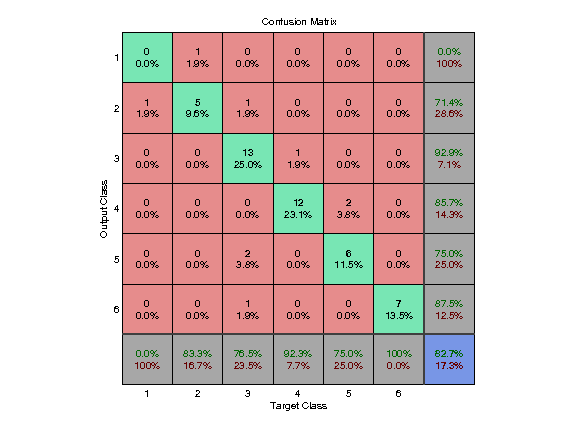
\includegraphics[scale=0.8]{../src/results/nominal/automobile_mc29.png}
				\caption{Matriz de confusión. Conjunto de datos Automobile. Clasificación nominal.}
				\label{fig:nomaut}
			\end{figure}
			
			\subsubsection{Conjunto de datos Balance Scale}
			
			En la Tabla \ref{tab:nombal} se muestran los resultados individuales de las 30 ejecuciones del algoritmo de clasificación nominal mediante una red neuronal artificial no ordinal para el conjunto de datos Balance Scale, donde se muestra el número de ejecuciones, el CCR, el MAE, el número de neuronas en capa oculta calculado y el tiempo total de la ejecución.\\
			
			\begin{table}[!htbp]
				\centering
				\CSVtotabular{../src/results/nominal/balance.csv}{l|r|r|r|r|r|r}{%
					\bfseries numIter &
					\bfseries CCR &
					\bfseries MAE &
					\bfseries NH &
					\bfseries CompTime\\\hline}{%
					\insertnumIter &
					\insertCCR &
					\insertMAE &
					\insertNH &
					\insertCompTime\\}{%
					\insertnumIter &
					\insertCCR &
					\insertMAE &
					\insertNH &
					\insertCompTime\\
					}
				\caption{Resultados individuales. Conjunto de datos Balance Scale. Clasificación nominal.}
				\label{tab:nombal}
			\end{table}
			
			La matriz de confusión para el mejor resultado del CCR obtenido de las 30 ejecuciones es la que se muestra en la Figura \ref{fig:nombal}.
			
			\begin{figure}[htbp]
				\centering
				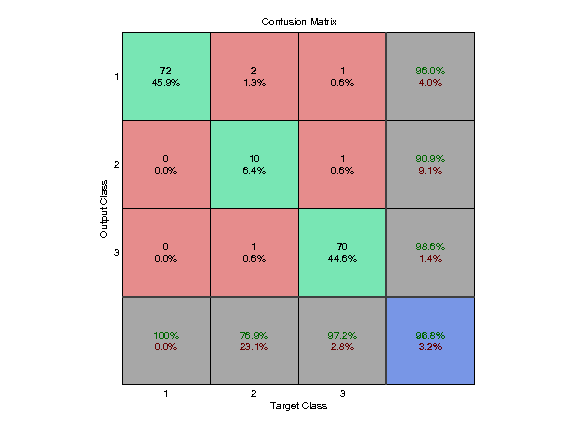
\includegraphics[scale=0.8]{../src/results/nominal/balance_mc6.png}
				\caption{Matriz de confusión. Conjunto de datos Balance Scale. Clasificación nominal.}
				\label{fig:nombal}
			\end{figure}
			
			\subsubsection{Conjunto de datos Bondrate}
			
			En la Tabla \ref{tab:nombon} se muestran los resultados individuales de las 30 ejecuciones del algoritmo de clasificación nominal mediante una red neuronal artificial no ordinal para el conjunto de datos Bondrate, donde se muestra el número de ejecuciones, el CCR, el MAE, el número de neuronas en capa oculta calculado y el tiempo total de la ejecución.\\
			
			\begin{table}[!htbp]
				\centering
				\CSVtotabular{../src/results/nominal/bondrate.csv}{l|r|r|r|r|r|r}{%
					\bfseries numIter &
					\bfseries CCR &
					\bfseries MAE &
					\bfseries NH &
					\bfseries CompTime\\\hline}{%
					\insertnumIter &
					\insertCCR &
					\insertMAE &
					\insertNH &
					\insertCompTime\\}{%
					\insertnumIter &
					\insertCCR &
					\insertMAE &
					\insertNH &
					\insertCompTime\\
					}
				\caption{Resultados individuales. Conjunto de datos Bondrate. Clasificación nominal.}
				\label{tab:nombon}
			\end{table}
			
			La matriz de confusión para el mejor resultado del CCR obtenido de las 30 ejecuciones es la que se muestra en la Figura \ref{fig:nombon}.
			
			\begin{figure}[htbp]
				\centering
				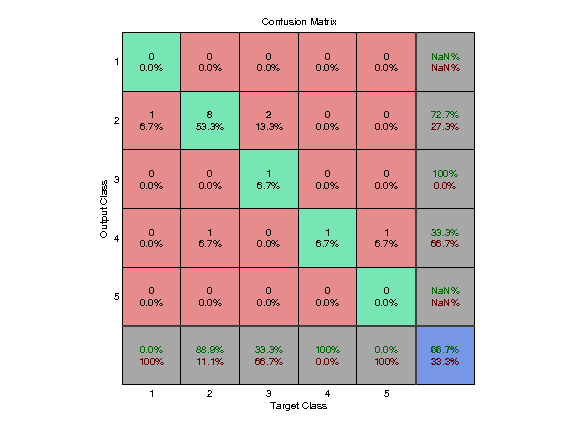
\includegraphics[scale=0.8]{../src/results/nominal/bondrate_mc1.png}
				\caption{Matriz de confusión. Conjunto de datos Bondrate. Clasificación nominal.}
				\label{fig:nombon}
			\end{figure}

			\subsubsection{Conjunto de datos Car}
			
			En la Tabla \ref{tab:nomcar} se muestran los resultados individuales de las 30 ejecuciones del algoritmo de clasificación nominal mediante una red neuronal artificial no ordinal para el conjunto de datos Car, donde se muestra el número de ejecuciones, el CCR, el MAE, el número de neuronas en capa oculta calculado y el tiempo total de la ejecución.\\
			
			\begin{table}[!htbp]
				\centering
				\CSVtotabular{../src/results/nominal/car.csv}{l|r|r|r|r|r|r}{%
					\bfseries numIter &
					\bfseries CCR &
					\bfseries MAE &
					\bfseries NH &
					\bfseries CompTime\\\hline}{%
					\insertnumIter &
					\insertCCR &
					\insertMAE &
					\insertNH &
					\insertCompTime\\}{%
					\insertnumIter &
					\insertCCR &
					\insertMAE &
					\insertNH &
					\insertCompTime\\
					}
				\caption{Resultados individuales. Conjunto de datos Car. Clasificación nominal.}
				\label{tab:nomcar}
			\end{table}
			
			La matriz de confusión para el mejor resultado del CCR obtenido de las 30 ejecuciones es la que se muestra en la Figura \ref{fig:nomcar}.
			
			\begin{figure}[htbp]
				\centering
				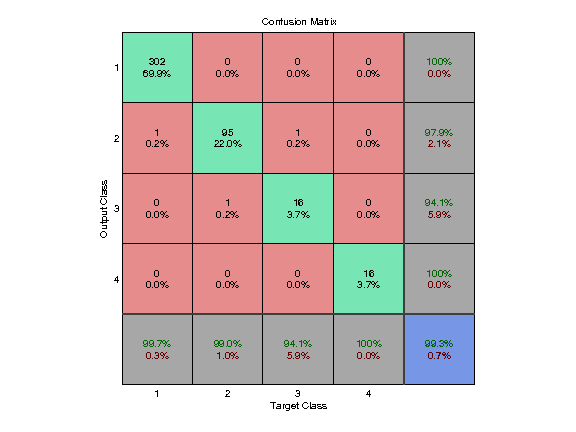
\includegraphics[scale=0.8]{../src/results/nominal/car_mc22.png}
				\caption{Matriz de confusión. Conjunto de datos Car. Clasificación nominal.}
				\label{fig:nomcar}
			\end{figure}

			\subsubsection{Conjunto de datos Contact lenses}
			
			En la Tabla \ref{tab:nomcon} se muestran los resultados individuales de las 30 ejecuciones del algoritmo de clasificación nominal mediante una red neuronal artificial no ordinal para el conjunto de datos Contact Lenses, donde se muestra el número de ejecuciones, el CCR, el MAE, el número de neuronas en capa oculta calculado y el tiempo total de la ejecución.\\
			
			\begin{table}[!htbp]
				\centering
				\CSVtotabular{../src/results/nominal/contact-lenses.csv}{l|r|r|r|r|r|r}{%
					\bfseries numIter &
					\bfseries CCR &
					\bfseries MAE &
					\bfseries NH &
					\bfseries CompTime\\\hline}{%
					\insertnumIter &
					\insertCCR &
					\insertMAE &
					\insertNH &
					\insertCompTime\\}{%
					\insertnumIter &
					\insertCCR &
					\insertMAE &
					\insertNH &
					\insertCompTime\\
					}
				\caption{Resultados individuales. Conjunto de datos Contact Lenses. Clasificación nominal.}
				\label{tab:nomcon}
			\end{table}
			
			La matriz de confusión para el mejor resultado del CCR obtenido de las 30 ejecuciones es la que se muestra en la Figura \ref{fig:nomcon}.
			
			\begin{figure}[htbp]
				\centering
				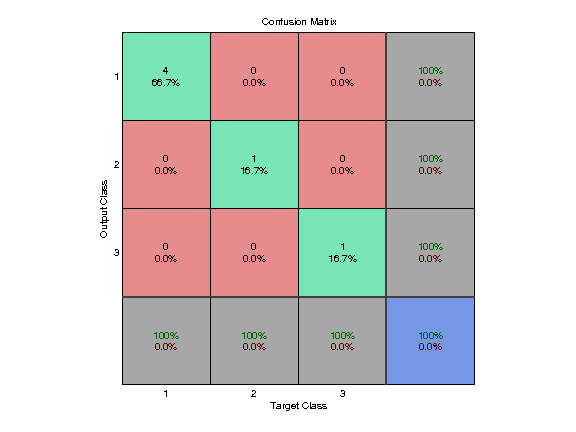
\includegraphics[scale=0.8]{../src/results/nominal/contact-lenses_mc2.png}
				\caption{Matriz de confusión. Conjunto de datos Contact Lenses. Clasificación nominal.}
				\label{fig:nomcon}
			\end{figure}

			\subsubsection{Conjunto de datos Depression}
			
			En la Tabla \ref{tab:nomdep} se muestran los resultados individuales de las 30 ejecuciones del algoritmo de clasificación nominal mediante una red neuronal artificial no ordinal para el conjunto de datos Depression, donde se muestra el número de ejecuciones, el CCR, el MAE, el número de neuronas en capa oculta calculado y el tiempo total de la ejecución.\\
			
			\begin{table}[!htbp]
				\centering
				\CSVtotabular{../src/results/nominal/depresion.csv}{l|r|r|r|r|r|r}{%
					\bfseries numIter &
					\bfseries CCR &
					\bfseries MAE &
					\bfseries NH &
					\bfseries CompTime\\\hline}{%
					\insertnumIter &
					\insertCCR &
					\insertMAE &
					\insertNH &
					\insertCompTime\\}{%
					\insertnumIter &
					\insertCCR &
					\insertMAE &
					\insertNH &
					\insertCompTime\\
					}
				\caption{Resultados individuales. Conjunto de datos Depression. Clasificación nominal.}
				\label{tab:nomdep}
			\end{table}
			
			La matriz de confusión para el mejor resultado del CCR obtenido de las 30 ejecuciones es la que se muestra en la Figura \ref{fig:nomdep}.
			
			\begin{figure}[htbp]
				\centering
				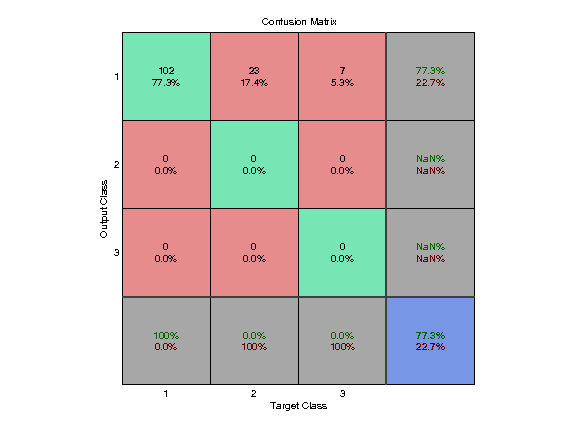
\includegraphics[scale=0.8]{../src/results/nominal/depresion_mc1.png}
				\caption{Matriz de confusión. Conjunto de datos Depression. Clasificación nominal.}
				\label{fig:nomdep}
			\end{figure}

			\subsubsection{Conjunto de datos ERA}
			
			En la Tabla \ref{tab:nomera} se muestran los resultados individuales de las 30 ejecuciones del algoritmo de clasificación nominal mediante una red neuronal artificial no ordinal para el conjunto de datos ERA, donde se muestra el número de ejecuciones, el CCR, el MAE, el número de neuronas en capa oculta calculado y el tiempo total de la ejecución.\\
			
			\begin{table}[!htbp]
				\centering
				\CSVtotabular{../src/results/nominal/ERA.csv}{l|r|r|r|r|r|r}{%
					\bfseries numIter &
					\bfseries CCR &
					\bfseries MAE &
					\bfseries NH &
					\bfseries CompTime\\\hline}{%
					\insertnumIter &
					\insertCCR &
					\insertMAE &
					\insertNH &
					\insertCompTime\\}{%
					\insertnumIter &
					\insertCCR &
					\insertMAE &
					\insertNH &
					\insertCompTime\\
					}
				\caption{Resultados individuales. Conjunto de datos ERA. Clasificación nominal.}
				\label{tab:nomera}
			\end{table}
			
			La matriz de confusión para el mejor resultado del CCR obtenido de las 30 ejecuciones es la que se muestra en la Figura \ref{fig:nomera}.
			
			\begin{figure}[htbp]
				\centering
				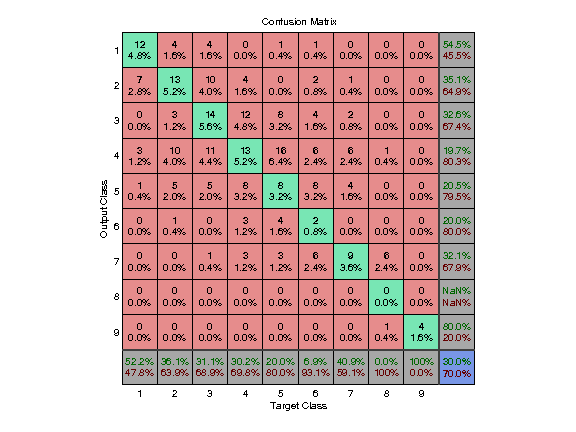
\includegraphics[scale=0.8]{../src/results/nominal/ERA_mc2.png}
				\caption{Matriz de confusión. Conjunto de datos ERA. Clasificación nominal.}
				\label{fig:nomera}
			\end{figure}

			\subsubsection{Conjunto de datos ESL}
			
			En la Tabla \ref{tab:nomesl} se muestran los resultados individuales de las 30 ejecuciones del algoritmo de clasificación nominal mediante una red neuronal artificial no ordinal para el conjunto de datos ESL, donde se muestra el número de ejecuciones, el CCR, el MAE, el número de neuronas en capa oculta calculado y el tiempo total de la ejecución.\\
			
			\begin{table}[!htbp]
				\centering
				\CSVtotabular{../src/results/nominal/ESL.csv}{l|r|r|r|r|r|r}{%
					\bfseries numIter &
					\bfseries CCR &
					\bfseries MAE &
					\bfseries NH &
					\bfseries CompTime\\\hline}{%
					\insertnumIter &
					\insertCCR &
					\insertMAE &
					\insertNH &
					\insertCompTime\\}{%
					\insertnumIter &
					\insertCCR &
					\insertMAE &
					\insertNH &
					\insertCompTime\\
					}
				\caption{Resultados individuales. Conjunto de datos ESL. Clasificación nominal.}
				\label{tab:nomesl}
			\end{table}
			
			La matriz de confusión para el mejor resultado del CCR obtenido de las 30 ejecuciones es la que se muestra en la Figura \ref{fig:nomesl}.
			
			\begin{figure}[htbp]
				\centering
				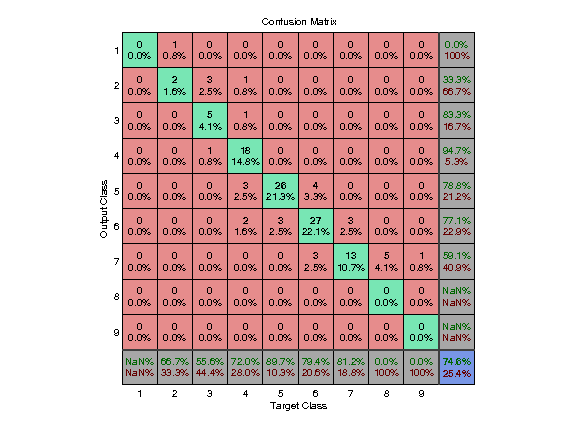
\includegraphics[scale=0.8]{../src/results/nominal/ESL_mc12.png}
				\caption{Matriz de confusión. Conjunto de datos ESL. Clasificación nominal.}
				\label{fig:nomesl}
			\end{figure}

			\subsubsection{Conjunto de datos Eucalyptus}
			
			En la Tabla \ref{tab:nomeuc} se muestran los resultados individuales de las 30 ejecuciones del algoritmo de clasificación nominal mediante una red neuronal artificial no ordinal para el conjunto de datos Eucalyptus, donde se muestra el número de ejecuciones, el CCR, el MAE, el número de neuronas en capa oculta calculado y el tiempo total de la ejecución.\\
			
			\begin{table}[!htbp]
				\centering
				\CSVtotabular{../src/results/nominal/eucalyptus.csv}{l|r|r|r|r|r|r}{%
					\bfseries numIter &
					\bfseries CCR &
					\bfseries MAE &
					\bfseries NH &
					\bfseries CompTime\\\hline}{%
					\insertnumIter &
					\insertCCR &
					\insertMAE &
					\insertNH &
					\insertCompTime\\}{%
					\insertnumIter &
					\insertCCR &
					\insertMAE &
					\insertNH &
					\insertCompTime\\
					}
				\caption{Resultados individuales. Conjunto de datos Eucalyptus. Clasificación nominal.}
				\label{tab:nomeuc}
			\end{table}
			
			La matriz de confusión para el mejor resultado del CCR obtenido de las 30 ejecuciones es la que se muestra en la Figura \ref{fig:nomeuc}.
			
			\begin{figure}[htbp]
				\centering
				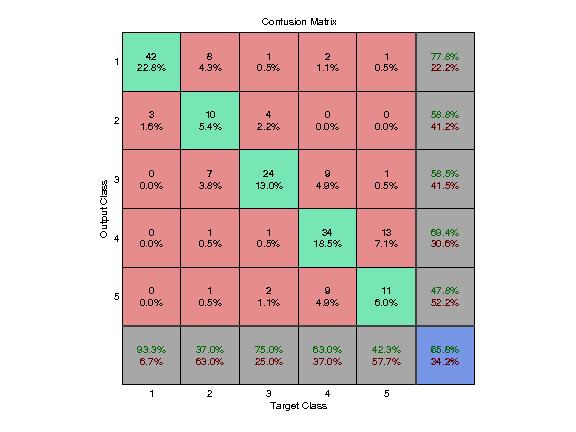
\includegraphics[scale=0.8]{../src/results/nominal/eucalyptus_mc1.png}
				\caption{Matriz de confusión. Conjunto de datos Eucalyptus. Clasificación nominal.}
				\label{fig:nomeuc}
			\end{figure}

			\subsubsection{Conjunto de datos LEV}
			
			En la Tabla \ref{tab:nomlev} se muestran los resultados individuales de las 30 ejecuciones del algoritmo de clasificación nominal mediante una red neuronal artificial no ordinal para el conjunto de datos LEV, donde se muestra el número de ejecuciones, el CCR, el MAE, el número de neuronas en capa oculta calculado y el tiempo total de la ejecución.\\
			
			\begin{table}[!htbp]
				\centering
				\CSVtotabular{../src/results/nominal/LEV.csv}{l|r|r|r|r|r|r}{%
					\bfseries numIter &
					\bfseries CCR &
					\bfseries MAE &
					\bfseries NH &
					\bfseries CompTime\\\hline}{%
					\insertnumIter &
					\insertCCR &
					\insertMAE &
					\insertNH &
					\insertCompTime\\}{%
					\insertnumIter &
					\insertCCR &
					\insertMAE &
					\insertNH &
					\insertCompTime\\
					}
				\caption{Resultados individuales. Conjunto de datos LEV. Clasificación nominal.}
				\label{tab:nomlev}
			\end{table}
			
			La matriz de confusión para el mejor resultado del CCR obtenido de las 30 ejecuciones es la que se muestra en la Figura \ref{fig:nomlev}.
			
			\begin{figure}[htbp]
				\centering
				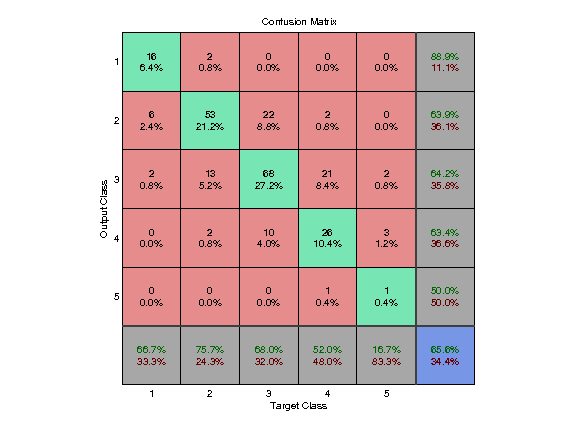
\includegraphics[scale=0.8]{../src/results/nominal/LEV_mc28.png}
				\caption{Matriz de confusión. Conjunto de datos LEV. Clasificación nominal.}
				\label{fig:nomlev}
			\end{figure}

			\subsubsection{Conjunto de datos New Thyroid}
			
			En la Tabla \ref{tab:nomnew} se muestran los resultados individuales de las 30 ejecuciones del algoritmo de clasificación nominal mediante una red neuronal artificial no ordinal para el conjunto de datos New Thyroid, donde se muestra el número de ejecuciones, el CCR, el MAE, el número de neuronas en capa oculta calculado y el tiempo total de la ejecución.\\
			
			\begin{table}[!htbp]
				\centering
				\CSVtotabular{../src/results/nominal/newthyroid.csv}{l|r|r|r|r|r|r}{%
					\bfseries numIter &
					\bfseries CCR &
					\bfseries MAE &
					\bfseries NH &
					\bfseries CompTime\\\hline}{%
					\insertnumIter &
					\insertCCR &
					\insertMAE &
					\insertNH &
					\insertCompTime\\}{%
					\insertnumIter &
					\insertCCR &
					\insertMAE &
					\insertNH &
					\insertCompTime\\
					}
				\caption{Resultados individuales. Conjunto de datos New Thyroid. Clasificación nominal.}
				\label{tab:nomnew}
			\end{table}
			
			La matriz de confusión para el mejor resultado del CCR obtenido de las 30 ejecuciones es la que se muestra en la Figura \ref{fig:nomnew}.
			
			\begin{figure}[htbp]
				\centering
				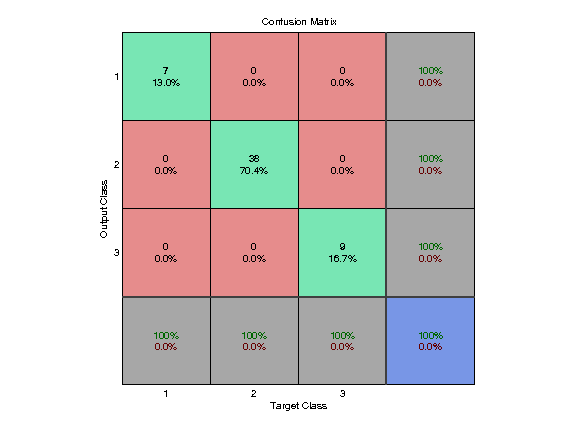
\includegraphics[scale=0.8]{../src/results/nominal/newthyroid_mc14.png}
				\caption{Matriz de confusión. Conjunto de datos New Thyroid. Clasificación nominal.}
				\label{fig:nomnew}
			\end{figure}

			\subsubsection{Conjunto de datos Pasture}
			
			En la Tabla \ref{tab:nompas} se muestran los resultados individuales de las 30 ejecuciones del algoritmo de clasificación nominal mediante una red neuronal artificial no ordinal para el conjunto de datos Pasture, donde se muestra el número de ejecuciones, el CCR, el MAE, el número de neuronas en capa oculta calculado y el tiempo total de la ejecución.\\
			
			\begin{table}[!htbp]
				\centering
				\CSVtotabular{../src/results/nominal/pasture.csv}{l|r|r|r|r|r|r}{%
					\bfseries numIter &
					\bfseries CCR &
					\bfseries MAE &
					\bfseries NH &
					\bfseries CompTime\\\hline}{%
					\insertnumIter &
					\insertCCR &
					\insertMAE &
					\insertNH &
					\insertCompTime\\}{%
					\insertnumIter &
					\insertCCR &
					\insertMAE &
					\insertNH &
					\insertCompTime\\
					}
				\caption{Resultados individuales. Conjunto de datos Pasture. Clasificación nominal.}
				\label{tab:nompas}
			\end{table}
			
			La matriz de confusión para el mejor resultado del CCR obtenido de las 30 ejecuciones es la que se muestra en la Figura \ref{fig:nompas}.
			
			\begin{figure}[htbp]
				\centering
				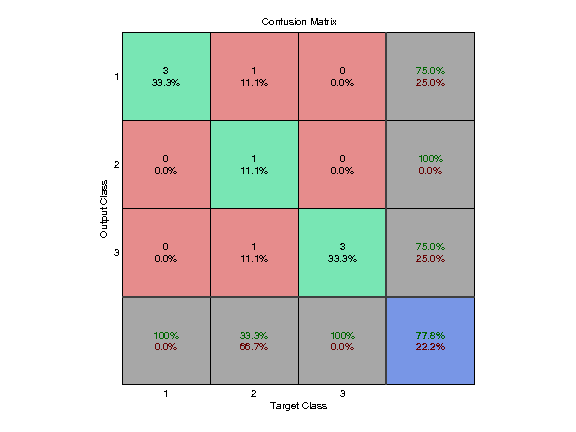
\includegraphics[scale=0.8]{../src/results/nominal/pasture_mc7.png}
				\caption{Matriz de confusión. Conjunto de datos Pasture. Clasificación nominal.}
				\label{fig:nompas}
			\end{figure}

			\subsubsection{Conjunto de datos Squash Stored}
			
			En la Tabla \ref{tab:nomsqu} se muestran los resultados individuales de las 30 ejecuciones del algoritmo de clasificación nominal mediante una red neuronal artificial no ordinal para el conjunto de datos Squash Stored, donde se muestra el número de ejecuciones, el CCR, el MAE, el número de neuronas en capa oculta calculado y el tiempo total de la ejecución.\\
			
			\begin{table}[!htbp]
				\centering
				\CSVtotabular{../src/results/nominal/squash-stored.csv}{l|r|r|r|r|r|r}{%
					\bfseries numIter &
					\bfseries CCR &
					\bfseries MAE &
					\bfseries NH &
					\bfseries CompTime\\\hline}{%
					\insertnumIter &
					\insertCCR &
					\insertMAE &
					\insertNH &
					\insertCompTime\\}{%
					\insertnumIter &
					\insertCCR &
					\insertMAE &
					\insertNH &
					\insertCompTime\\
					}
				\caption{Resultados individuales. Conjunto de datos Squash Stored. Clasificación nominal.}
				\label{tab:nomsqu}
			\end{table}
			
			La matriz de confusión para el mejor resultado del CCR obtenido de las 30 ejecuciones es la que se muestra en la Figura \ref{fig:nomsqu}.
			
			\begin{figure}[htbp]
				\centering
				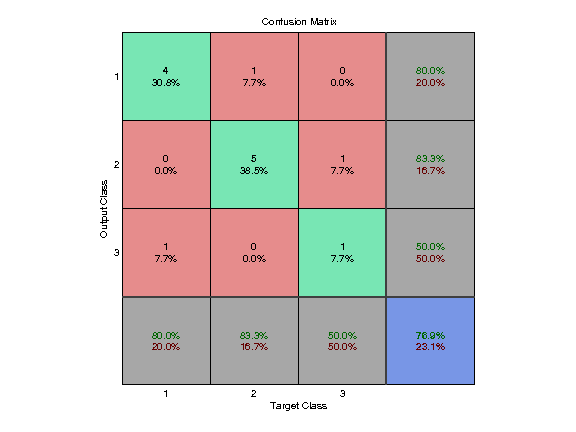
\includegraphics[scale=0.8]{../src/results/nominal/squash-stored_mc25.png}
				\caption{Matriz de confusión. Conjunto de datos Squash Stored. Clasificación nominal.}
				\label{fig:nomsqu}
			\end{figure}

			\subsubsection{Conjunto de datos Squash Unstored}
			
			En la Tabla \ref{tab:nomsqua} se muestran los resultados individuales de las 30 ejecuciones del algoritmo de clasificación nominal mediante una red neuronal artificial no ordinal para el conjunto de datos Squash Unstored, donde se muestra el número de ejecuciones, el CCR, el MAE, el número de neuronas en capa oculta calculado y el tiempo total de la ejecución.\\
			
			\begin{table}[!htbp]
				\centering
				\CSVtotabular{../src/results/nominal/squash-unstored.csv}{l|r|r|r|r|r|r}{%
					\bfseries numIter &
					\bfseries CCR &
					\bfseries MAE &
					\bfseries NH &
					\bfseries CompTime\\\hline}{%
					\insertnumIter &
					\insertCCR &
					\insertMAE &
					\insertNH &
					\insertCompTime\\}{%
					\insertnumIter &
					\insertCCR &
					\insertMAE &
					\insertNH &
					\insertCompTime\\
					}
				\caption{Resultados individuales. Conjunto de datos Squash Unstored. Clasificación nominal.}
				\label{tab:nomsqua}
			\end{table}
			
			La matriz de confusión para el mejor resultado del CCR obtenido de las 30 ejecuciones es la que se muestra en la Figura \ref{fig:nomsqua}.
			
			\begin{figure}[htbp]
				\centering
				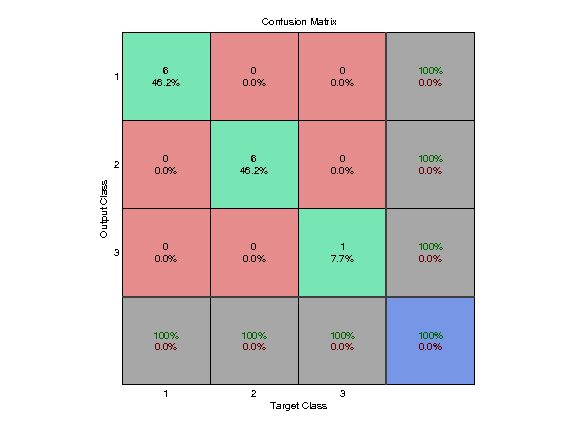
\includegraphics[scale=0.8]{../src/results/nominal/squash-unstored_mc20.png}
				\caption{Matriz de confusión. Conjunto de datos Squash Unstored. Clasificación nominal.}
				\label{fig:nomsqua}
			\end{figure}

			\subsubsection{Conjunto de datos SWD}
			
			En la Tabla \ref{tab:nomswd} se muestran los resultados individuales de las 30 ejecuciones del algoritmo de clasificación nominal mediante una red neuronal artificial no ordinal para el conjunto de datos SWD, donde se muestra el número de ejecuciones, el CCR, el MAE, el número de neuronas en capa oculta calculado y el tiempo total de la ejecución.\\
			
			\begin{table}[!htbp]
				\centering
				\CSVtotabular{../src/results/nominal/SWD.csv}{l|r|r|r|r|r|r}{%
					\bfseries numIter &
					\bfseries CCR &
					\bfseries MAE &
					\bfseries NH &
					\bfseries CompTime\\\hline}{%
					\insertnumIter &
					\insertCCR &
					\insertMAE &
					\insertNH &
					\insertCompTime\\}{%
					\insertnumIter &
					\insertCCR &
					\insertMAE &
					\insertNH &
					\insertCompTime\\
					}
				\caption{Resultados individuales. Conjunto de datos SWD. Clasificación nominal.}
				\label{tab:nomswd}
			\end{table}
			
			La matriz de confusión para el mejor resultado del CCR obtenido de las 30 ejecuciones es la que se muestra en la Figura \ref{fig:nomswd}.
			
			\begin{figure}[htbp]
				\centering
				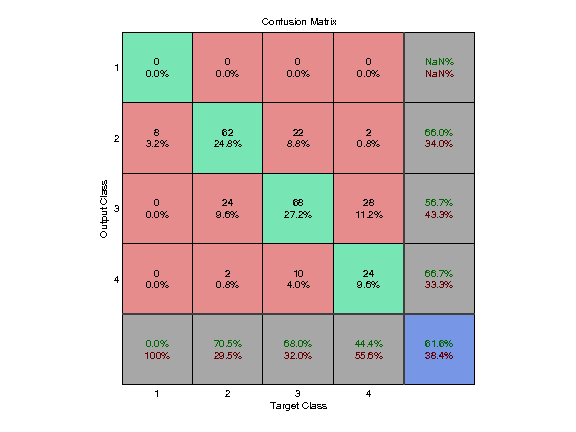
\includegraphics[scale=0.8]{../src/results/nominal/SWD_mc7.png}
				\caption{Matriz de confusión. Conjunto de datos SWD. Clasificación nominal.}
				\label{fig:nomswd}
			\end{figure}

			\subsubsection{Conjunto de datos TAE}
			
			En la Tabla \ref{tab:nomtae} se muestran los resultados individuales de las 30 ejecuciones del algoritmo de clasificación nominal mediante una red neuronal artificial no ordinal para el conjunto de datos TAE, donde se muestra el número de ejecuciones, el CCR, el MAE, el número de neuronas en capa oculta calculado y el tiempo total de la ejecución.\\
			
			\begin{table}[!htbp]
				\centering
				\CSVtotabular{../src/results/nominal/tae.csv}{l|r|r|r|r|r|r}{%
					\bfseries numIter &
					\bfseries CCR &
					\bfseries MAE &
					\bfseries NH &
					\bfseries CompTime\\\hline}{%
					\insertnumIter &
					\insertCCR &
					\insertMAE &
					\insertNH &
					\insertCompTime\\}{%
					\insertnumIter &
					\insertCCR &
					\insertMAE &
					\insertNH &
					\insertCompTime\\
					}
				\caption{Resultados individuales. Conjunto de datos TAE. Clasificación nominal.}
				\label{tab:nomtae}
			\end{table}
			
			La matriz de confusión para el mejor resultado del CCR obtenido de las 30 ejecuciones es la que se muestra en la Figura \ref{fig:nomtae}.
			
			\begin{figure}[htbp]
				\centering
				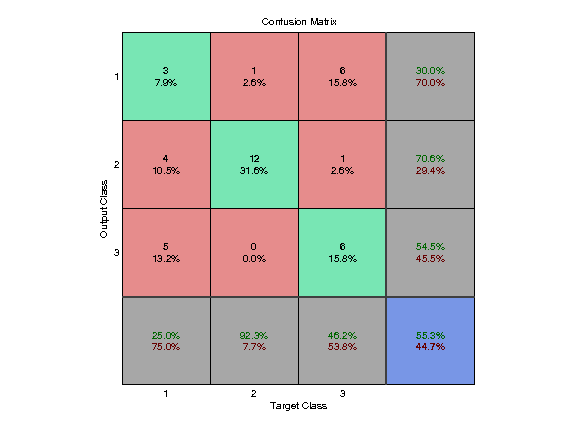
\includegraphics[scale=0.8]{../src/results/nominal/tae_mc16.png}
				\caption{Matriz de confusión. Conjunto de datos TAE. Clasificación nominal.}
				\label{fig:nomtae}
			\end{figure}

			\subsubsection{Conjunto de datos Thyroid}
			
			En la Tabla \ref{tab:nomthy} se muestran los resultados individuales de las 30 ejecuciones del algoritmo de clasificación nominal mediante una red neuronal artificial no ordinal para el conjunto de datos Thyroid, donde se muestra el número de ejecuciones, el CCR, el MAE, el número de neuronas en capa oculta calculado y el tiempo total de la ejecución.\\
			
			\begin{table}[!htbp]
				\centering
				\CSVtotabular{../src/results/nominal/thyroid.csv}{l|r|r|r|r|r|r}{%
					\bfseries numIter &
					\bfseries CCR &
					\bfseries MAE &
					\bfseries NH &
					\bfseries CompTime\\\hline}{%
					\insertnumIter &
					\insertCCR &
					\insertMAE &
					\insertNH &
					\insertCompTime\\}{%
					\insertnumIter &
					\insertCCR &
					\insertMAE &
					\insertNH &
					\insertCompTime\\
					}
				\caption{Resultados individuales. Conjunto de datos Thyroid. Clasificación nominal.}
				\label{tab:nomthy}
			\end{table}
			
			La matriz de confusión para el mejor resultado del CCR obtenido de las 30 ejecuciones es la que se muestra en la Figura \ref{fig:nomthy}.
			
			\begin{figure}[htbp]
				\centering
				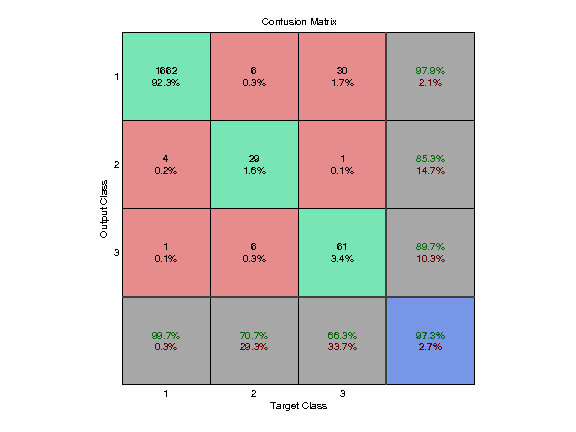
\includegraphics[scale=0.8]{../src/results/nominal/thyroid_mc29.png}
				\caption{Matriz de confusión. Conjunto de datos Thyroid. Clasificación nominal.}
				\label{fig:nomthy}
			\end{figure}

			\subsubsection{Conjunto de datos Wine Quality Red}
			
			En la Tabla \ref{tab:nomred} se muestran los resultados individuales de las 30 ejecuciones del algoritmo de clasificación nominal mediante una red neuronal artificial no ordinal para el conjunto de datos Wine Quality Red, donde se muestra el número de ejecuciones, el CCR, el MAE, el número de neuronas en capa oculta calculado y el tiempo total de la ejecución.\\
			
			\begin{table}[!htbp]
				\centering
				\CSVtotabular{../src/results/nominal/winequality-red.csv}{l|r|r|r|r|r|r}{%
					\bfseries numIter &
					\bfseries CCR &
					\bfseries MAE &
					\bfseries NH &
					\bfseries CompTime\\\hline}{%
					\insertnumIter &
					\insertCCR &
					\insertMAE &
					\insertNH &
					\insertCompTime\\}{%
					\insertnumIter &
					\insertCCR &
					\insertMAE &
					\insertNH &
					\insertCompTime\\
					}
				\caption{Resultados individuales. Conjunto de datos Wine Quality Red. Clasificación nominal.}
				\label{tab:nomred}
			\end{table}
			
			La matriz de confusión para el mejor resultado del CCR obtenido de las 30 ejecuciones es la que se muestra en la Figura \ref{fig:nomred}.
			
			\begin{figure}[htbp]
				\centering
				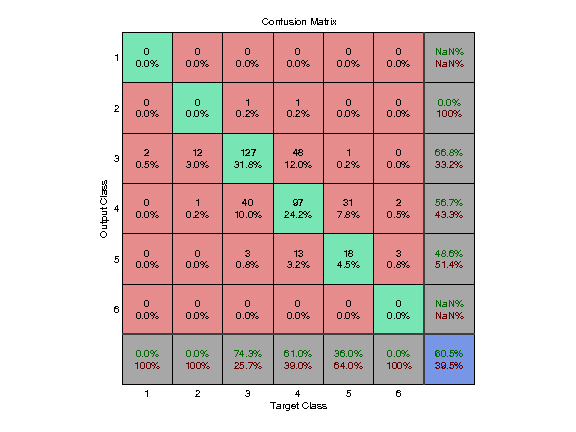
\includegraphics[scale=0.8]{../src/results/nominal/winequality-red_mc1.png}
				\caption{Matriz de confusión. Conjunto de datos Wine Quality Red. Clasificación nominal.}
				\label{fig:nomred}
			\end{figure}

			\subsubsection{Conjunto de datos Wine Quality White}
			
			En la Tabla \ref{tab:nomwhi} se muestran los resultados individuales de las 30 ejecuciones del algoritmo de clasificación nominal mediante una red neuronal artificial no ordinal para el conjunto de datos Wine Quality White, donde se muestra el número de ejecuciones, el CCR, el MAE, el número de neuronas en capa oculta calculado y el tiempo total de la ejecución.\\
			
			\begin{table}[!htbp]
				\centering
				\CSVtotabular{../src/results/nominal/winequality-white.csv}{l|r|r|r|r|r|r}{%
					\bfseries numIter &
					\bfseries CCR &
					\bfseries MAE &
					\bfseries NH &
					\bfseries CompTime\\\hline}{%
					\insertnumIter &
					\insertCCR &
					\insertMAE &
					\insertNH &
					\insertCompTime\\}{%
					\insertnumIter &
					\insertCCR &
					\insertMAE &
					\insertNH &
					\insertCompTime\\
					}
				\caption{Resultados individuales. Conjunto de datos Wine Quality White. Clasificación nominal.}
				\label{tab:nomwhi}
			\end{table}
			
			La matriz de confusión para el mejor resultado del CCR obtenido de las 30 ejecuciones es la que se muestra en la Figura \ref{fig:nomwhi}.
			
			\begin{figure}[htbp]
				\centering
				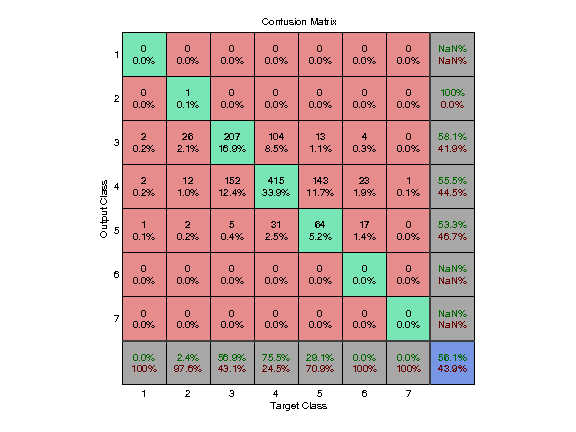
\includegraphics[scale=0.8]{../src/results/nominal/winequality-white_mc14.png}
				\caption{Matriz de confusión. Conjunto de datos Wine Quality White. Clasificación nominal.}
				\label{fig:nomwhi}
			\end{figure}
		
		\subsection{Clasificación Ordinal}
		
			Para cada uno de los conjuntos se mostrarán los datos obtenidos correspondientes a aplicar un modelo de clasificación donde se tiene en cuenta el orden de las etiquetas y la matriz de confusión del mejor resultado.
	
			\subsubsection{Conjunto de datos Automobile}
			
			En la Tabla \ref{tab:ordaut} se muestran los resultados individuales de las 30 ejecuciones del algoritmo de regresión ordinal ORNNet mediante una red neuronal artificial ordinal para el conjunto de datos Automobile, donde se muestra el número de ejecuciones, el CCR, el MAE, el número de neuronas en capa oculta calculado y el tiempo total de la ejecución.\\
			
			\begin{table}[!htbp]
				\centering
				\CSVtotabular{../src/results/ordinal/automobile.csv}{l|r|r|r|r|r|r}{%
					\bfseries numIter &
					\bfseries CCR &
					\bfseries MAE &
					\bfseries NH &
					\bfseries CompTime\\\hline}{%
					\insertnumIter &
					\insertCCR &
					\insertMAE &
					\insertNH &
					\insertCompTime\\}{%
					\insertnumIter &
					\insertCCR &
					\insertMAE &
					\insertNH &
					\insertCompTime\\
					}
				\caption{Resultados individuales. Conjunto de datos Automobile. Clasificación ordinal.}
				\label{tab:ordaut}
			\end{table}
			
			La matriz de confusión para el mejor resultado del CCR obtenido de las 30 ejecuciones es la que se muestra en la Figura \ref{fig:ordaut}.
			
			\begin{figure}[htbp]
				\centering
				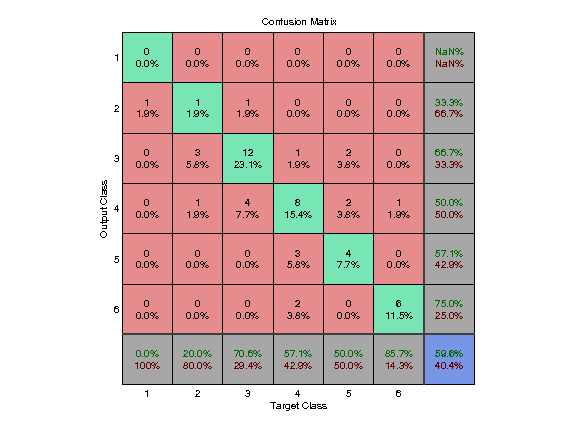
\includegraphics[scale=0.8]{../src/results/ordinal/automobile_mc1.png}
				\caption{Matriz de confusión. Conjunto de datos Automobile. Clasificación ordinal.}
				\label{fig:ordaut}
			\end{figure}
			
			\subsubsection{Conjunto de datos Balance Scale}
			
			En la Tabla \ref{tab:ordbal} se muestran los resultados individuales de las 30 ejecuciones del algoritmo de regresión ordinal ORNNet mediante una red neuronal artificial ordinal para el conjunto de datos Balance Scale, donde se muestra el número de ejecuciones, el CCR, el MAE, el número de neuronas en capa oculta calculado y el tiempo total de la ejecución.\\
			
			\begin{table}[!htbp]
				\centering
				\CSVtotabular{../src/results/ordinal/balance.csv}{l|r|r|r|r|r|r}{%
					\bfseries numIter &
					\bfseries CCR &
					\bfseries MAE &
					\bfseries NH &
					\bfseries CompTime\\\hline}{%
					\insertnumIter &
					\insertCCR &
					\insertMAE &
					\insertNH &
					\insertCompTime\\}{%
					\insertnumIter &
					\insertCCR &
					\insertMAE &
					\insertNH &
					\insertCompTime\\
					}
				\caption{Resultados individuales. Conjunto de datos Balance Scale. Clasificación ordinal.}
				\label{tab:ordbal}
			\end{table}
			
			La matriz de confusión para el mejor resultado del CCR obtenido de las 30 ejecuciones es la que se muestra en la Figura \ref{fig:ordbal}.
			
			\begin{figure}[htbp]
				\centering
				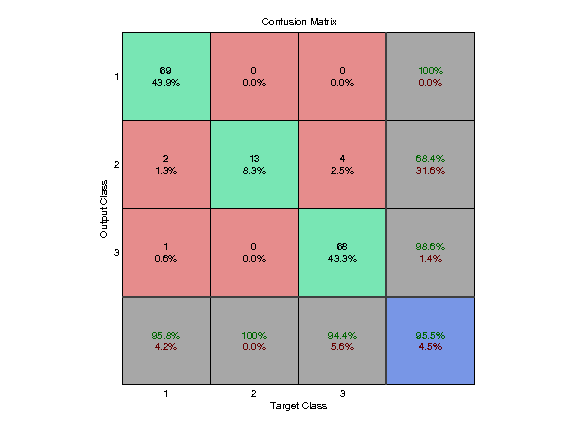
\includegraphics[scale=0.8]{../src/results/ordinal/balance_mc1.png}
				\caption{Matriz de confusión. Conjunto de datos Balance Scale. Clasificación ordinal.}
				\label{fig:ordbal}
			\end{figure}
			
			\subsubsection{Conjunto de datos Bondrate}
			
			En la Tabla \ref{tab:ordbon} se muestran los resultados individuales de las 30 ejecuciones del algoritmo de regresión ordinal ORNNet mediante una red neuronal artificial ordinal para el conjunto de datos Bondrate, donde se muestra el número de ejecuciones, el CCR, el MAE, el número de neuronas en capa oculta calculado y el tiempo total de la ejecución.\\
			
			\begin{table}[!htbp]
				\centering
				\CSVtotabular{../src/results/ordinal/bondrate.csv}{l|r|r|r|r|r|r}{%
					\bfseries numIter &
					\bfseries CCR &
					\bfseries MAE &
					\bfseries NH &
					\bfseries CompTime\\\hline}{%
					\insertnumIter &
					\insertCCR &
					\insertMAE &
					\insertNH &
					\insertCompTime\\}{%
					\insertnumIter &
					\insertCCR &
					\insertMAE &
					\insertNH &
					\insertCompTime\\
					}
				\caption{Resultados individuales. Conjunto de datos Bondrate. Clasificación ordinal.}
				\label{tab:ordbon}
			\end{table}
			
			La matriz de confusión para el mejor resultado del CCR obtenido de las 30 ejecuciones es la que se muestra en la Figura \ref{fig:ordbon}.
			
			\begin{figure}[htbp]
				\centering
				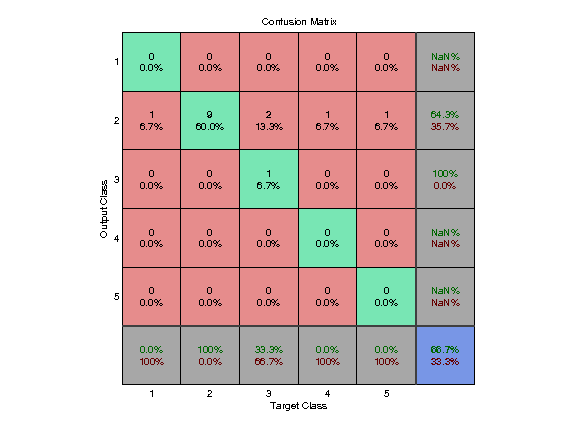
\includegraphics[scale=0.8]{../src/results/ordinal/bondrate_mc1.png}
				\caption{Matriz de confusión. Conjunto de datos Bondrate. Clasificación ordinal.}
				\label{fig:ordbon}
			\end{figure}
			
			\subsubsection{Conjunto de datos Car}
			
			En la Tabla \ref{tab:ordcar} se muestran los resultados individuales de las 30 ejecuciones del algoritmo de regresión ordinal ORNNet mediante una red neuronal artificial ordinal para el conjunto de datos Car, donde se muestra el número de ejecuciones, el CCR, el MAE, el número de neuronas en capa oculta calculado y el tiempo total de la ejecución.\\
			
			\begin{table}[!htbp]
				\centering
				\CSVtotabular{../src/results/ordinal/car.csv}{l|r|r|r|r|r|r}{%
					\bfseries numIter &
					\bfseries CCR &
					\bfseries MAE &
					\bfseries NH &
					\bfseries CompTime\\\hline}{%
					\insertnumIter &
					\insertCCR &
					\insertMAE &
					\insertNH &
					\insertCompTime\\}{%
					\insertnumIter &
					\insertCCR &
					\insertMAE &
					\insertNH &
					\insertCompTime\\
					}
				\caption{Resultados individuales. Conjunto de datos Car. Clasificación ordinal.}
				\label{tab:ordcar}
			\end{table}
			
			La matriz de confusión para el mejor resultado del CCR obtenido de las 30 ejecuciones es la que se muestra en la Figura \ref{fig:ordcar}.
			
			\begin{figure}[htbp]
				\centering
				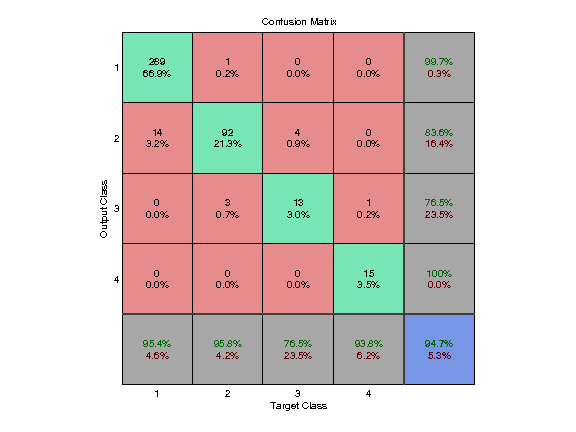
\includegraphics[scale=0.8]{../src/results/ordinal/car_mc1.png}
				\caption{Matriz de confusión. Conjunto de datos CAR. Clasificación ordinal.}
				\label{fig:ordcar}
			\end{figure}
			
			\subsubsection{Conjunto de datos Contact lenses}
			
			En la Tabla \ref{tab:ordcon} se muestran los resultados individuales de las 30 ejecuciones del algoritmo de regresión ordinal ORNNet mediante una red neuronal artificial ordinal para el conjunto de datos Contact Lenses, donde se muestra el número de ejecuciones, el CCR, el MAE, el número de neuronas en capa oculta calculado y el tiempo total de la ejecución.\\
			
			\begin{table}[!htbp]
				\centering
				\CSVtotabular{../src/results/ordinal/contact-lenses.csv}{l|r|r|r|r|r|r}{%
					\bfseries numIter &
					\bfseries CCR &
					\bfseries MAE &
					\bfseries NH &
					\bfseries CompTime\\\hline}{%
					\insertnumIter &
					\insertCCR &
					\insertMAE &
					\insertNH &
					\insertCompTime\\}{%
					\insertnumIter &
					\insertCCR &
					\insertMAE &
					\insertNH &
					\insertCompTime\\
					}
				\caption{Resultados individuales. Conjunto de datos Contact Lenses. Clasificación ordinal.}
				\label{tab:ordcon}
			\end{table}
			
			La matriz de confusión para el mejor resultado del CCR obtenido de las 30 ejecuciones es la que se muestra en la Figura \ref{fig:ordcon}.
			
			\begin{figure}[htbp]
				\centering
				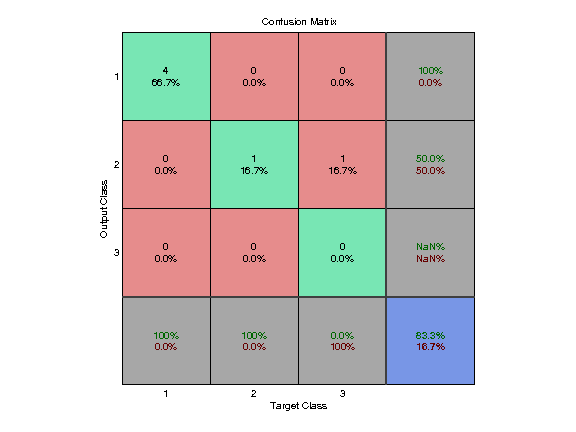
\includegraphics[scale=0.8]{../src/results/ordinal/contact-lenses_mc1.png}
				\caption{Matriz de confusión. Conjunto de datos Contact Lenses. Clasificación ordinal.}
				\label{fig:ordcon}
			\end{figure}
			
			\subsubsection{Conjunto de datos Depression}
			
			En la Tabla \ref{tab:orddep} se muestran los resultados individuales de las 30 ejecuciones del algoritmo de regresión ordinal ORNNet mediante una red neuronal artificial ordinal para el conjunto de datos Depression, donde se muestra el número de ejecuciones, el CCR, el MAE, el número de neuronas en capa oculta calculado y el tiempo total de la ejecución.\\
			
			\begin{table}[!htbp]
				\centering
				\CSVtotabular{../src/results/ordinal/depresion.csv}{l|r|r|r|r|r|r}{%
					\bfseries numIter &
					\bfseries CCR &
					\bfseries MAE &
					\bfseries NH &
					\bfseries CompTime\\\hline}{%
					\insertnumIter &
					\insertCCR &
					\insertMAE &
					\insertNH &
					\insertCompTime\\}{%
					\insertnumIter &
					\insertCCR &
					\insertMAE &
					\insertNH &
					\insertCompTime\\
					}
				\caption{Resultados individuales. Conjunto de datos Depression. Clasificación ordinal.}
				\label{tab:orddep}
			\end{table}
			
			La matriz de confusión para el mejor resultado del CCR obtenido de las 30 ejecuciones es la que se muestra en la Figura \ref{fig:orddep}.
			
			\begin{figure}[htbp]
				\centering
				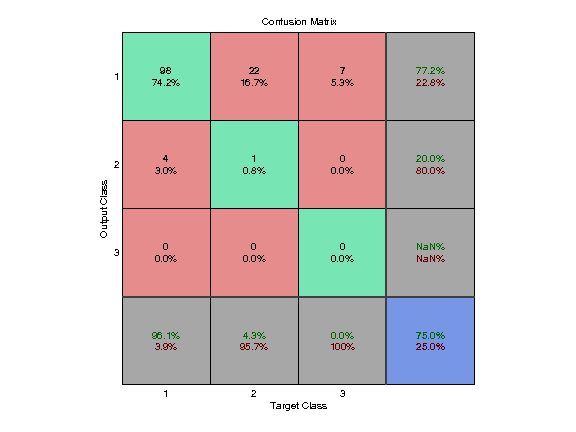
\includegraphics[scale=0.8]{../src/results/ordinal/depresion_mc1.png}
				\caption{Matriz de confusión. Conjunto de datos Depression. Clasificación ordinal.}
				\label{fig:orddep}
			\end{figure}
			
			\subsubsection{Conjunto de datos ERA}
			
			En la Tabla \ref{tab:ordera} se muestran los resultados individuales de las 30 ejecuciones del algoritmo de regresión ordinal ORNNet mediante una red neuronal artificial ordinal para el conjunto de datos ERA, donde se muestra el número de ejecuciones, el CCR, el MAE, el número de neuronas en capa oculta calculado y el tiempo total de la ejecución.\\
			
			\begin{table}[!htbp]
				\centering
				\CSVtotabular{../src/results/ordinal/ERA.csv}{l|r|r|r|r|r|r}{%
					\bfseries numIter &
					\bfseries CCR &
					\bfseries MAE &
					\bfseries NH &
					\bfseries CompTime\\\hline}{%
					\insertnumIter &
					\insertCCR &
					\insertMAE &
					\insertNH &
					\insertCompTime\\}{%
					\insertnumIter &
					\insertCCR &
					\insertMAE &
					\insertNH &
					\insertCompTime\\
					}
				\caption{Resultados individuales. Conjunto de datos ERA. Clasificación ordinal.}
				\label{tab:ordera}
			\end{table}
			
			La matriz de confusión para el mejor resultado del CCR obtenido de las 30 ejecuciones es la que se muestra en la Figura \ref{fig:ordera}.
			
			\begin{figure}[htbp]
				\centering
				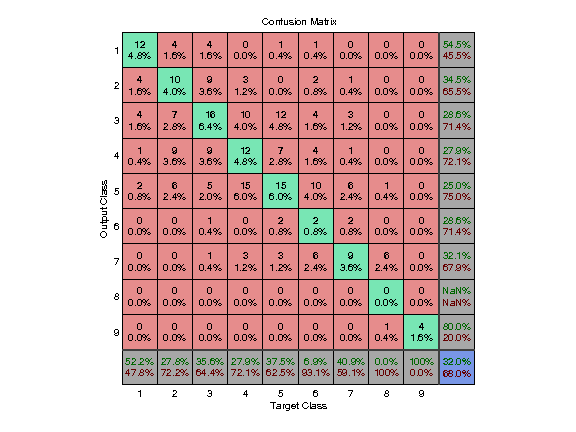
\includegraphics[scale=0.8]{../src/results/ordinal/ERA_mc1.png}
				\caption{Matriz de confusión. Conjunto de datos ERA. Clasificación ordinal.}
				\label{fig:ordera}
			\end{figure}
			
			\subsubsection{Conjunto de datos ESL}
			
			En la Tabla \ref{tab:ordesl} se muestran los resultados individuales de las 30 ejecuciones del algoritmo de regresión ordinal ORNNet mediante una red neuronal artificial ordinal para el conjunto de datos ESL, donde se muestra el número de ejecuciones, el CCR, el MAE, el número de neuronas en capa oculta calculado y el tiempo total de la ejecución.\\
			
			\begin{table}[!htbp]
				\centering
				\CSVtotabular{../src/results/ordinal/ESL.csv}{l|r|r|r|r|r|r}{%
					\bfseries numIter &
					\bfseries CCR &
					\bfseries MAE &
					\bfseries NH &
					\bfseries CompTime\\\hline}{%
					\insertnumIter &
					\insertCCR &
					\insertMAE &
					\insertNH &
					\insertCompTime\\}{%
					\insertnumIter &
					\insertCCR &
					\insertMAE &
					\insertNH &
					\insertCompTime\\
					}
				\caption{Resultados individuales. Conjunto de datos ESL. Clasificación ordinal.}
				\label{tab:ordesl}
			\end{table}
			
			La matriz de confusión para el mejor resultado del CCR obtenido de las 30 ejecuciones es la que se muestra en la Figura \ref{fig:ordesl}.
			
			\begin{figure}[htbp]
				\centering
				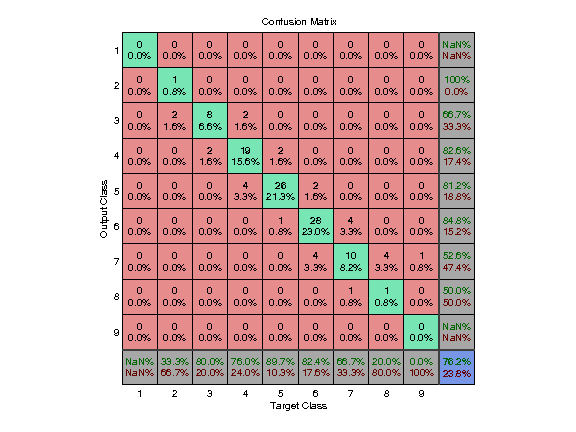
\includegraphics[scale=0.8]{../src/results/ordinal/ESL_mc1.png}
				\caption{Matriz de confusión. Conjunto de datos ESL. Clasificación ordinal.}
				\label{fig:ordesl}
			\end{figure}
			
			\subsubsection{Conjunto de datos Eucalyptus}
			
			En la Tabla \ref{tab:ordeuc} se muestran los resultados individuales de las 30 ejecuciones del algoritmo de regresión ordinal ORNNet mediante una red neuronal artificial ordinal para el conjunto de datos Eucalyptus, donde se muestra el número de ejecuciones, el CCR, el MAE, el número de neuronas en capa oculta calculado y el tiempo total de la ejecución.\\
			
			\begin{table}[!htbp]
				\centering
				\CSVtotabular{../src/results/ordinal/eucalyptus.csv}{l|r|r|r|r|r|r}{%
					\bfseries numIter &
					\bfseries CCR &
					\bfseries MAE &
					\bfseries NH &
					\bfseries CompTime\\\hline}{%
					\insertnumIter &
					\insertCCR &
					\insertMAE &
					\insertNH &
					\insertCompTime\\}{%
					\insertnumIter &
					\insertCCR &
					\insertMAE &
					\insertNH &
					\insertCompTime\\
					}
				\caption{Resultados individuales. Conjunto de datos Eucalyptus. Clasificación ordinal.}
				\label{tab:ordeuc}
			\end{table}
			
			La matriz de confusión para el mejor resultado del CCR obtenido de las 30 ejecuciones es la que se muestra en la Figura \ref{fig:ordeuc}.
			
			\begin{figure}[htbp]
				\centering
				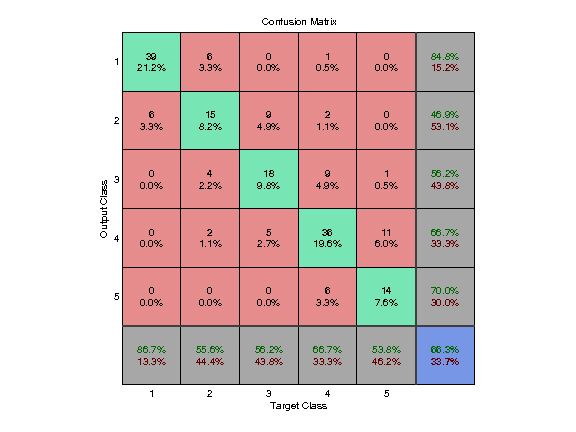
\includegraphics[scale=0.8]{../src/results/ordinal/eucalyptus_mc1.png}
				\caption{Matriz de confusión. Conjunto de datos Eucalyptus. Clasificación ordinal.}
				\label{fig:ordeuc}
			\end{figure}
			
			\subsubsection{Conjunto de datos LEV}
			
			En la Tabla \ref{tab:ordlev} se muestran los resultados individuales de las 30 ejecuciones del algoritmo de regresión ordinal ORNNet mediante una red neuronal artificial ordinal para el conjunto de datos LEV, donde se muestra el número de ejecuciones, el CCR, el MAE, el número de neuronas en capa oculta calculado y el tiempo total de la ejecución.\\
			
			\begin{table}[!htbp]
				\centering
				\CSVtotabular{../src/results/ordinal/LEV.csv}{l|r|r|r|r|r|r}{%
					\bfseries numIter &
					\bfseries CCR &
					\bfseries MAE &
					\bfseries NH &
					\bfseries CompTime\\\hline}{%
					\insertnumIter &
					\insertCCR &
					\insertMAE &
					\insertNH &
					\insertCompTime\\}{%
					\insertnumIter &
					\insertCCR &
					\insertMAE &
					\insertNH &
					\insertCompTime\\
					}
				\caption{Resultados individuales. Conjunto de datos LEV. Clasificación ordinal.}
				\label{tab:ordlev}
			\end{table}
			
			La matriz de confusión para el mejor resultado del CCR obtenido de las 30 ejecuciones es la que se muestra en la Figura \ref{fig:ordlev}.
			
			\begin{figure}[htbp]
				\centering
				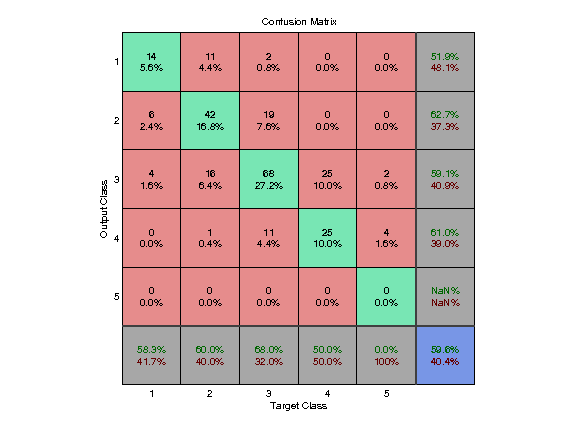
\includegraphics[scale=0.8]{../src/results/ordinal/LEV_mc1.png}
				\caption{Matriz de confusión. Conjunto de datos LEV. Clasificación ordinal.}
				\label{fig:ordlev}
			\end{figure}
			
			\subsubsection{Conjunto de datos New Thyroid}
			
			En la Tabla \ref{tab:ordnew} se muestran los resultados individuales de las 30 ejecuciones del algoritmo de regresión ordinal ORNNet mediante una red neuronal artificial ordinal para el conjunto de datos New Thyroid, donde se muestra el número de ejecuciones, el CCR, el MAE, el número de neuronas en capa oculta calculado y el tiempo total de la ejecución.\\
			
			\begin{table}[!htbp]
				\centering
				\CSVtotabular{../src/results/ordinal/newthyroid.csv}{l|r|r|r|r|r|r}{%
					\bfseries numIter &
					\bfseries CCR &
					\bfseries MAE &
					\bfseries NH &
					\bfseries CompTime\\\hline}{%
					\insertnumIter &
					\insertCCR &
					\insertMAE &
					\insertNH &
					\insertCompTime\\}{%
					\insertnumIter &
					\insertCCR &
					\insertMAE &
					\insertNH &
					\insertCompTime\\
					}
				\caption{Resultados individuales. Conjunto de datos New Thyroid. Clasificación ordinal.}
				\label{tab:ordnew}
			\end{table}
			
			La matriz de confusión para el mejor resultado del CCR obtenido de las 30 ejecuciones es la que se muestra en la Figura \ref{fig:ordnew}.
			
			\begin{figure}[htbp]
				\centering
				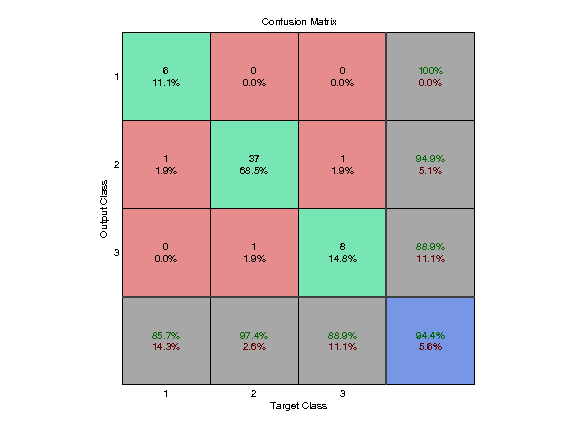
\includegraphics[scale=0.8]{../src/results/ordinal/newthyroid_mc1.png}
				\caption{Matriz de confusión. Conjunto de datos New Thyroid. Clasificación ordinal.}
				\label{fig:ordnew}
			\end{figure}
			
			\subsubsection{Conjunto de datos Pasture}
			
			En la Tabla \ref{tab:ordpas} se muestran los resultados individuales de las 30 ejecuciones del algoritmo de regresión ordinal ORNNet mediante una red neuronal artificial ordinal para el conjunto de datos Pasture, donde se muestra el número de ejecuciones, el CCR, el MAE, el número de neuronas en capa oculta calculado y el tiempo total de la ejecución.\\
			
			\begin{table}[!htbp]
				\centering
				\CSVtotabular{../src/results/ordinal/pasture.csv}{l|r|r|r|r|r|r}{%
					\bfseries numIter &
					\bfseries CCR &
					\bfseries MAE &
					\bfseries NH &
					\bfseries CompTime\\\hline}{%
					\insertnumIter &
					\insertCCR &
					\insertMAE &
					\insertNH &
					\insertCompTime\\}{%
					\insertnumIter &
					\insertCCR &
					\insertMAE &
					\insertNH &
					\insertCompTime\\
					}
				\caption{Resultados individuales. Conjunto de datos Pasture. Clasificación ordinal.}
				\label{tab:ordpas}
			\end{table}
			
			La matriz de confusión para el mejor resultado del CCR obtenido de las 30 ejecuciones es la que se muestra en la Figura \ref{fig:ordpas}.
			
			\begin{figure}[htbp]
				\centering
				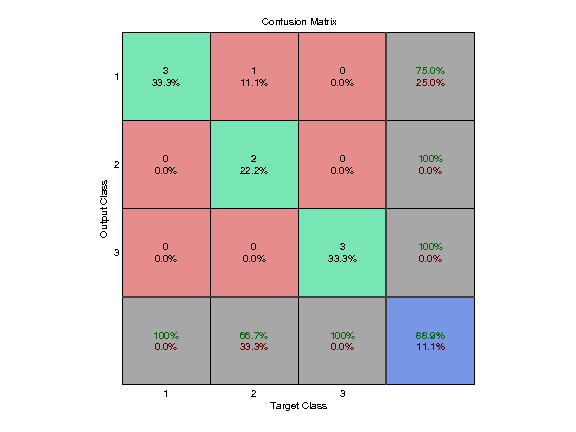
\includegraphics[scale=0.8]{../src/results/ordinal/pasture_mc1.png}
				\caption{Matriz de confusión. Conjunto de datos Pasture. Clasificación ordinal.}
				\label{fig:ordpas}
			\end{figure}
			
			\subsubsection{Conjunto de datos Squash Stored}
			
			En la Tabla \ref{tab:ordsqu} se muestran los resultados individuales de las 30 ejecuciones del algoritmo de regresión ordinal ORNNet mediante una red neuronal artificial ordinal para el conjunto de datos Squash Stored, donde se muestra el número de ejecuciones, el CCR, el MAE, el número de neuronas en capa oculta calculado y el tiempo total de la ejecución.\\
			
			\begin{table}[!htbp]
				\centering
				\CSVtotabular{../src/results/ordinal/squash-stored.csv}{l|r|r|r|r|r|r}{%
					\bfseries numIter &
					\bfseries CCR &
					\bfseries MAE &
					\bfseries NH &
					\bfseries CompTime\\\hline}{%
					\insertnumIter &
					\insertCCR &
					\insertMAE &
					\insertNH &
					\insertCompTime\\}{%
					\insertnumIter &
					\insertCCR &
					\insertMAE &
					\insertNH &
					\insertCompTime\\
					}
				\caption{Resultados individuales. Conjunto de datos Squash Stored. Clasificación ordinal.}
				\label{tab:ordsqu}
			\end{table}
			
			La matriz de confusión para el mejor resultado del CCR obtenido de las 30 ejecuciones es la que se muestra en la Figura \ref{fig:ordsqu}.
			
			\begin{figure}[htbp]
				\centering
				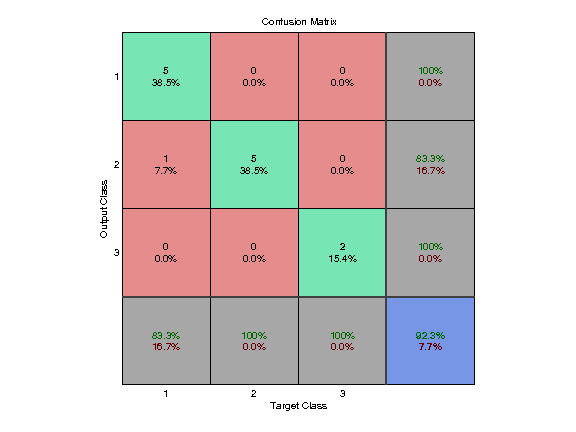
\includegraphics[scale=0.8]{../src/results/ordinal/squash-stored_mc1.png}
				\caption{Matriz de confusión. Conjunto de datos Squash Stored. Clasificación ordinal.}
				\label{fig:ordsqu}
			\end{figure}
			
			\subsubsection{Conjunto de datos Squash Unstored}
			
			En la Tabla \ref{tab:ordsqua} se muestran los resultados individuales de las 30 ejecuciones del algoritmo de regresión ordinal ORNNet mediante una red neuronal artificial ordinal para el conjunto de datos Squash Unstored, donde se muestra el número de ejecuciones, el CCR, el MAE, el número de neuronas en capa oculta calculado y el tiempo total de la ejecución.\\
			
			\begin{table}[!htbp]
				\centering
				\CSVtotabular{../src/results/ordinal/squash-unstored.csv}{l|r|r|r|r|r|r}{%
					\bfseries numIter &
					\bfseries CCR &
					\bfseries MAE &
					\bfseries NH &
					\bfseries CompTime\\\hline}{%
					\insertnumIter &
					\insertCCR &
					\insertMAE &
					\insertNH &
					\insertCompTime\\}{%
					\insertnumIter &
					\insertCCR &
					\insertMAE &
					\insertNH &
					\insertCompTime\\
					}
				\caption{Resultados individuales. Conjunto de datos Squash Unstored. Clasificación ordinal.}
				\label{tab:ordsqua}
			\end{table}
			
			La matriz de confusión para el mejor resultado del CCR obtenido de las 30 ejecuciones es la que se muestra en la Figura \ref{fig:ordsqua}.
			
			\begin{figure}[htbp]
				\centering
				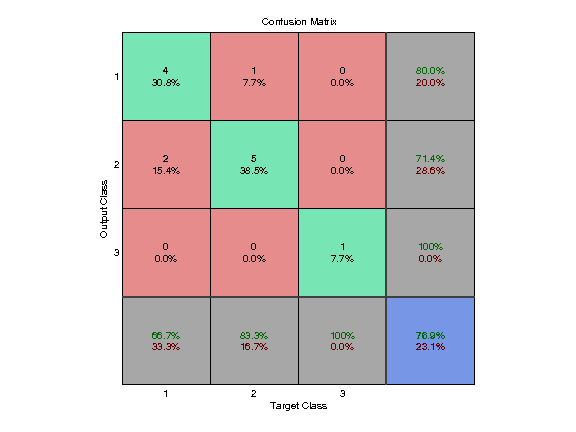
\includegraphics[scale=0.8]{../src/results/ordinal/squash-unstored_mc1.png}
				\caption{Matriz de confusión. Conjunto de datos Squash Unstored. Clasificación ordinal.}
				\label{fig:ordsqua}
			\end{figure}
			
			\subsubsection{Conjunto de datos SWD}
			
			En la Tabla \ref{tab:ordswd} se muestran los resultados individuales de las 30 ejecuciones del algoritmo de regresión ordinal ORNNet mediante una red neuronal artificial ordinal para el conjunto de datos SWD, donde se muestra el número de ejecuciones, el CCR, el MAE, el número de neuronas en capa oculta calculado y el tiempo total de la ejecución.\\
			
			\begin{table}[!htbp]
				\centering
				\CSVtotabular{../src/results/ordinal/SWD.csv}{l|r|r|r|r|r|r}{%
					\bfseries numIter &
					\bfseries CCR &
					\bfseries MAE &
					\bfseries NH &
					\bfseries CompTime\\\hline}{%
					\insertnumIter &
					\insertCCR &
					\insertMAE &
					\insertNH &
					\insertCompTime\\}{%
					\insertnumIter &
					\insertCCR &
					\insertMAE &
					\insertNH &
					\insertCompTime\\
					}
				\caption{Resultados individuales. Conjunto de datos SWD. Clasificación ordinal.}
				\label{tab:ordswd}
			\end{table}
			
			La matriz de confusión para el mejor resultado del CCR obtenido de las 30 ejecuciones es la que se muestra en la Figura \ref{fig:ordswd}.
			
			\begin{figure}[htbp]
				\centering
				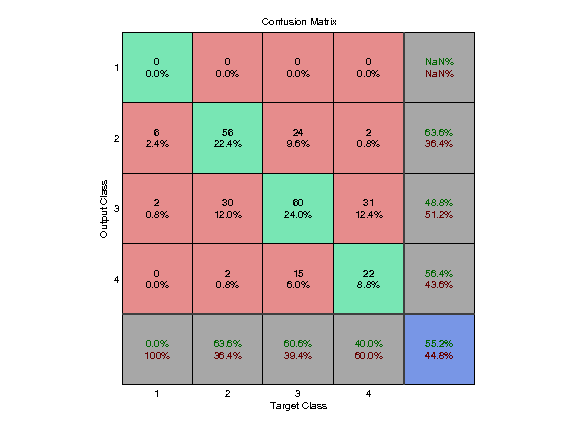
\includegraphics[scale=0.8]{../src/results/ordinal/SWD_mc1.png}
				\caption{Matriz de confusión. Conjunto de datos SWD. Clasificación ordinal.}
				\label{fig:ordswd}
			\end{figure}
			
			\subsubsection{Conjunto de datos TAE}
			
			En la Tabla \ref{tab:ordtae} se muestran los resultados individuales de las 30 ejecuciones del algoritmo de regresión ordinal ORNNet mediante una red neuronal artificial ordinal para el conjunto de datos TAE, donde se muestra el número de ejecuciones, el CCR, el MAE, el número de neuronas en capa oculta calculado y el tiempo total de la ejecución.\\
			
			\begin{table}[!htbp]
				\centering
				\CSVtotabular{../src/results/ordinal/tae.csv}{l|r|r|r|r|r|r}{%
					\bfseries numIter &
					\bfseries CCR &
					\bfseries MAE &
					\bfseries NH &
					\bfseries CompTime\\\hline}{%
					\insertnumIter &
					\insertCCR &
					\insertMAE &
					\insertNH &
					\insertCompTime\\}{%
					\insertnumIter &
					\insertCCR &
					\insertMAE &
					\insertNH &
					\insertCompTime\\
					}
				\caption{Resultados individuales. Conjunto de datos TAE. Clasificación ordinal.}
				\label{tab:ordtae}
			\end{table}
			
			La matriz de confusión para el mejor resultado del CCR obtenido de las 30 ejecuciones es la que se muestra en la Figura \ref{fig:ordtae}.
			
			\begin{figure}[htbp]
				\centering
				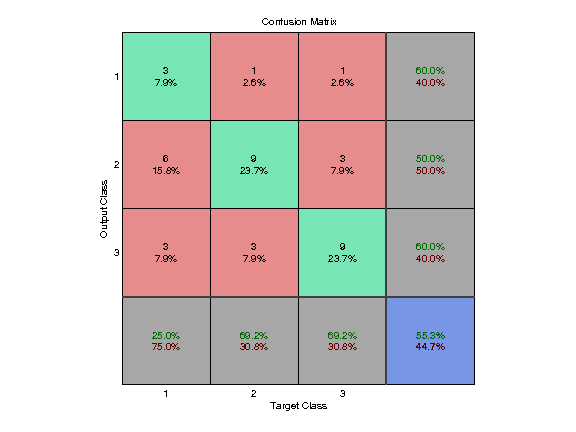
\includegraphics[scale=0.8]{../src/results/ordinal/tae_mc1.png}
				\caption{Matriz de confusión. Conjunto de datos TAE. Clasificación ordinal.}
				\label{fig:ordtae}
			\end{figure}
			
			\subsubsection{Conjunto de datos Thyroid}
			
			En la Tabla \ref{tab:ordthy} se muestran los resultados individuales de las 30 ejecuciones del algoritmo de regresión ordinal ORNNet mediante una red neuronal artificial ordinal para el conjunto de datos Thyroid, donde se muestra el número de ejecuciones, el CCR, el MAE, el número de neuronas en capa oculta calculado y el tiempo total de la ejecución.\\
			
			\begin{table}[!htbp]
				\centering
				\CSVtotabular{../src/results/ordinal/thyroid.csv}{l|r|r|r|r|r|r}{%
					\bfseries numIter &
					\bfseries CCR &
					\bfseries MAE &
					\bfseries NH &
					\bfseries CompTime\\\hline}{%
					\insertnumIter &
					\insertCCR &
					\insertMAE &
					\insertNH &
					\insertCompTime\\}{%
					\insertnumIter &
					\insertCCR &
					\insertMAE &
					\insertNH &
					\insertCompTime\\
					}
				\caption{Resultados individuales. Conjunto de datos Thyroid. Clasificación ordinal.}
				\label{tab:ordthy}
			\end{table}
			
			La matriz de confusión para el mejor resultado del CCR obtenido de las 30 ejecuciones es la que se muestra en la Figura \ref{fig:ordthy}.
			
			\begin{figure}[htbp]
				\centering
				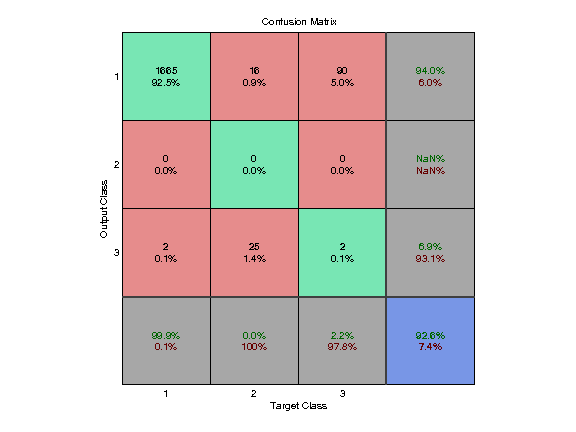
\includegraphics[scale=0.8]{../src/results/ordinal/thyroid_mc1.png}
				\caption{Matriz de confusión. Conjunto de datos Thyroid. Clasificación ordinal.}
				\label{fig:ordthy}
			\end{figure}
			
			\subsubsection{Conjunto de datos Wine Quality Red}
			
			En la Tabla \ref{tab:ordred} se muestran los resultados individuales de las 30 ejecuciones del algoritmo de regresión ordinal ORNNet mediante una red neuronal artificial ordinal para el conjunto de datos Wine Quality Red, donde se muestra el número de ejecuciones, el CCR, el MAE, el número de neuronas en capa oculta calculado y el tiempo total de la ejecución.\\
			
			\begin{table}[!htbp]
				\centering
				\CSVtotabular{../src/results/ordinal/winequality-red.csv}{l|r|r|r|r|r|r}{%
					\bfseries numIter &
					\bfseries CCR &
					\bfseries MAE &
					\bfseries NH &
					\bfseries CompTime\\\hline}{%
					\insertnumIter &
					\insertCCR &
					\insertMAE &
					\insertNH &
					\insertCompTime\\}{%
					\insertnumIter &
					\insertCCR &
					\insertMAE &
					\insertNH &
					\insertCompTime\\
					}
				\caption{Resultados individuales. Conjunto de datos Wine Quality Red. Clasificación ordinal.}
				\label{tab:ordred}
			\end{table}
			
			La matriz de confusión para el mejor resultado del CCR obtenido de las 30 ejecuciones es la que se muestra en la Figura \ref{fig:ordred}.
			
			\begin{figure}[htbp]
				\centering
				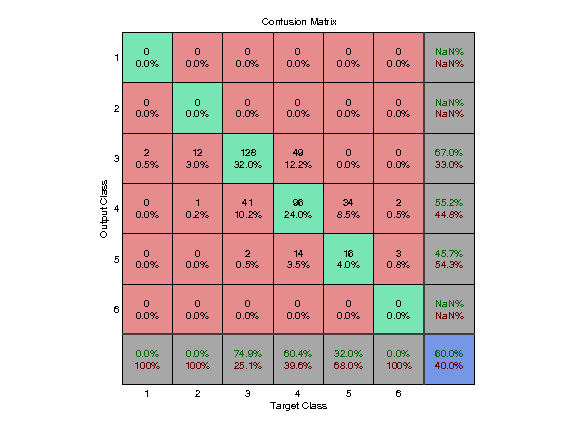
\includegraphics[scale=0.8]{../src/results/ordinal/winequality-red_mc1.png}
				\caption{Matriz de confusión. Conjunto de datos Wine Quality Red. Clasificación ordinal.}
				\label{fig:ordred}
			\end{figure}
			
			\subsubsection{Conjunto de datos Wine Quality White}
			
			En la Tabla \ref{tab:ordwhi} se muestran los resultados individuales de las 30 ejecuciones del algoritmo de regresión ordinal ORNNet mediante una red neuronal artificial ordinal para el conjunto de datos Wine Quality White, donde se muestra el número de ejecuciones, el CCR, el MAE, el número de neuronas en capa oculta calculado y el tiempo total de la ejecución.\\
			
			\begin{table}[!htbp]
				\centering
				\CSVtotabular{../src/results/ordinal/winequality-white.csv}{l|r|r|r|r|r|r}{%
					\bfseries numIter &
					\bfseries CCR &
					\bfseries MAE &
					\bfseries NH &
					\bfseries CompTime\\\hline}{%
					\insertnumIter &
					\insertCCR &
					\insertMAE &
					\insertNH &
					\insertCompTime\\}{%
					\insertnumIter &
					\insertCCR &
					\insertMAE &
					\insertNH &
					\insertCompTime\\
					}
				\caption{Resultados individuales. Conjunto de datos Wine Quality White. Clasificación ordinal.}
				\label{tab:ordwhi}
			\end{table}
			
			La matriz de confusión para el mejor resultado del CCR obtenido de las 30 ejecuciones es la que se muestra en la Figura \ref{fig:ordwhi}.
			
			\begin{figure}[htbp]
				\centering
				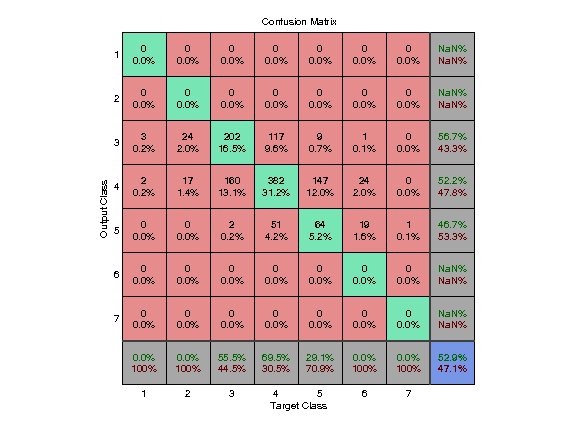
\includegraphics[scale=0.8]{../src/results/ordinal/winequality-white_mc1.png}
				\caption{Matriz de confusión. Conjunto de datos Wine Quality White. Clasificación ordinal.}
				\label{fig:ordwhi}
			\end{figure}
			
	\section{Resultados generales}
		
		Estos resultados son los obtenidos a partir de los resultados individuales, es decir, de cada uno de los conjuntos de datos se ha realizado la media y la desviación típica del CCR, el MAE y el NH.\\
		
		A partir de estos datos se podrá observar como de buenos son los resultados para una posterior comparativa.
		
		\subsection{Clasificación Nominal}
		
			La Tabla \ref{tab:gennom} muestra los resultados generales para los conjuntos de datos aplicando la clasificación nominal para la creación de la red neuronal y el entrenamiento y simulación.\\
		
			\begin{table}[!htbp]
				\centering
				\CSVtotabular{../src/results/nominal/general.csv}{l|r|r|r|r|r|r}{%
					\bfseries dataset &
					\bfseries CCRMean &
					\bfseries CCRSD &
					\bfseries MAEMean &
					\bfseries MAESD &
					\bfseries NHMean &
					\bfseries NHSD\\\hline}{%
					\insertdataset &
					\insertbyname{CCRMean} &
					\insertCCRSD &
					\insertMAEMean &
					\insertMAESD &
					\insertNHMean &
					\insertNHSD\\}{%
					\insertdataset &
					\insertbyname{CCRMean} &
					\insertCCRSD &
					\insertMAEMean &
					\insertMAESD &
					\insertNHMean &
					\insertNHSD\\
					}
				\caption{Resultados generales. Clasificación nominal.}
				\label{tab:gennom}
			\end{table}
		
		\subsection{Clasificación Ordinal}
		
			La Tabla \ref{tab:genord} muestra los resultados generales para los conjuntos de datos aplicando la clasificación ordinal para la creación de la red neuronal y el entrenamiento y simulación.
	
			\begin{table}[!htbp]
				\centering
				\CSVtotabular{../src/results/ordinal/general.csv}{l|r|r|r|r|r|r}{%
					\bfseries dataset &
					\bfseries CCRMean &
					\bfseries CCRSD &
					\bfseries MAEMean &
					\bfseries MAESD &
					\bfseries NHMean &
					\bfseries NHSD\\\hline}{%
					\insertdataset &
					\insertbyname{CCRMean} &
					\insertCCRSD &
					\insertMAEMean &
					\insertMAESD &
					\insertNHMean &
					\insertNHSD\\}{%
					\insertdataset &
					\insertbyname{CCRMean} &
					\insertCCRSD &
					\insertMAEMean &
					\insertMAESD &
					\insertNHMean &
					\insertNHSD\\
					}
				\caption{Resultados generales. Clasificación ordinal.}
				\label{tab:genord}
			\end{table}
	
	\section{Comparativa entre los resultados}
	
		En esta sección se hará un estudio comparativo entre las dos metodologías empleadas, nominal y ordinal, y de las cuales se podrán obtener las conclusiones en un capítulo posterior.\\
		
		Se hará una comparación entre los resultados generales de cada uno de las clasificaciones, observando y resaltando en cada caso cual ha sido mejor o peor para los conjuntos de datos evaluados. Para la comparativa entre los resultados obtenidos nos fijaremos en los valores medios del \textit{CCR} y del \textit{MAE}.\\
		
		Como se puede observar en la Tabla \ref{tab:comp}, los resultados obtenidos por el algoritmo ordinal ORNNet son mejores que para el algoritmo nominal, puesto que en 12 de los conjuntos de datos el \textit{CCR} es mayor que los resultados del algoritmo nominal y en 15 es menor el valor del \textit{MAE} para el ordinal. Además, en 11 la desviación típica es menor para el \textit{CCR} utilizando la clasificación ordinal frente a la nominal y en 14 también es menor la desviación típica para el \textit{MAE} utilizando la clasificación ordinal.
		
		\newpage{\thispagestyle{empty}}
		
		\begin{sidewaystable}[htbp]
			\centering
			\begin{tabular}{l|r|r|r|r|r|r|r|r}
				\cline{2-9}
				& \multicolumn{4}{c|}{\textbf{Nominal}} & \multicolumn{4}{c|}{\textbf{Ordinal}} \\
				\hline \textbf{dataset} & \textbf{CCRMean} & \textbf{CCRSD} & \textbf{MAEMean} & \textbf{MAESD} & \textbf{CCRMean} & \textbf{CCRSD} & \textbf{MAEMean} & \textbf{MAESD} \\ 
				\hline ERA & \cellcolor{myred} 0.249333 & 0.026623 & \cellcolor{myred} 1.360267 & 0.150086 & \cellcolor{mygreen} 0.267600 & 0.025415 & \cellcolor{mygreen} 1.240133 & 0.081750\\ 
				ESL & \cellcolor{myred} 0.694536 & 0.028794 & \cellcolor{myred} 0.329235 & 0.031200 & \cellcolor{mygreen} 0.714481 & 0.041744 & \cellcolor{mygreen} 0.302732 & 0.044685\\ 
				LEV & \cellcolor{myred} 0.598933 & 0.033564 & \cellcolor{myred} 0.431067 & 0.037665 & \cellcolor{mygreen} 0.607067 & 0.040936 & \cellcolor{mygreen} 0.419333 & 0.043490\\ 
				SWD & \cellcolor{myred} 0.561733 & 0.031839 & \cellcolor{myred} 0.467867 & 0.037294 & \cellcolor{mygreen} 0.567733 & 0.027270 & \cellcolor{mygreen} 0.451467 & 0.033855\\ 
				automobile & \cellcolor{myred} 0.600000 & 0.089548 & \cellcolor{myred} 0.580128 & 0.144536 & \cellcolor{mygreen} 0.641667 & 0.085480 & \cellcolor{mygreen} 0.443590 & 0.117023\\ 
				balance & \cellcolor{myred} 0.928662 & 0.026469 & \cellcolor{myred} 0.083864 & 0.034446 & \cellcolor{mygreen} 0.963907 & 0.018041 & \cellcolor{mygreen} 0.039066 & 0.019843\\ 
				bondrate & \cellcolor{myred} 0.560000 & 0.077509 & \cellcolor{myred} 0.606667 & 0.124229 & \cellcolor{mygreen} 0.568889 & 0.083475 & \cellcolor{mygreen} 0.584444 & 0.093765\\ 
				car & \cellcolor{mygreen} 0.977701 & 0.010900 & \cellcolor{mygreen} 0.025617 & 0.012634 & \cellcolor{myred} 0.968827 & 0.010955 & \cellcolor{myred} 0.031327 & 0.011039\\ 
				contact-lenses & \cellcolor{mygreen} 0.661111 & 0.202869 & \cellcolor{myred} 0.500000 & 0.327536 & \cellcolor{myred} 0.650000 & 0.153815 & \cellcolor{mygreen} 0.427778 & 0.184055\\ 
				depresion & \cellcolor{mygreen} 0.653283 & 0.192474 & \cellcolor{myred} 0.509091 & 0.316757 & \cellcolor{myred} 0.647475 & 0.149711 & \cellcolor{mygreen} 0.430808 & 0.179999\\ 
				eucalyptus & \cellcolor{myred} 0.599638 & 0.036704 & \cellcolor{myred} 0.476993 & 0.055290 & \cellcolor{mygreen} 0.650906 & 0.035615 & \cellcolor{mygreen} 0.385145 & 0.032663\\ 
				newthyroid & \cellcolor{myred} 0.956790 & 0.032014 & \cellcolor{myred} 0.043210 & 0.032014 & \cellcolor{mygreen} 0.964198 & 0.024284 & \cellcolor{mygreen} 0.035802 & 0.024284\\ 
				pasture & \cellcolor{mygreen} 0.722222 & 0.119421 & \cellcolor{mygreen} 0.311111 & 0.138101 & \cellcolor{myred} 0.648148 & 0.127468 & \cellcolor{myred} 0.351852 & 0.127468\\ 
				squash-stored & \cellcolor{myred} 0.656410 & 0.139567 & \cellcolor{myred} 0.366667 & 0.154750 & \cellcolor{mygreen} 0.661538 & 0.115340 & \cellcolor{mygreen} 0.353846 & 0.125507\\ 
				squash-unstored & \cellcolor{mygreen} 0.669231 & 0.131151 & \cellcolor{mygreen} 0.330769 & 0.131151 & \cellcolor{myred} 0.653846 & 0.156150 & \cellcolor{myred} 0.348718 & 0.160001\\ 
				tae & \cellcolor{myred} 0.414912 & 0.085952 & \cellcolor{myred} 0.764912 & 0.145938 & \cellcolor{mygreen} 0.441228 & 0.072047 & \cellcolor{mygreen} 0.648246 & 0.068233\\ 
				thyroid & \cellcolor{mygreen} 0.944630 & 0.008216 & \cellcolor{mygreen} 0.101574 & 0.015156 & \cellcolor{myred} 0.929426 & 0.006682 & \cellcolor{myred} 0.118352 & 0.013353\\ 
				winequality-red & \cellcolor{myred} 0.578250 & 0.016856 & \cellcolor{myred} 0.459833 & 0.020128 & \cellcolor{mygreen} 0.580833 & 0.020754 & \cellcolor{mygreen} 0.449917 & 0.022993\\ 
				winequality-white & \cellcolor{mygreen} 0.543728 & 0.010689 & \cellcolor{myred} 0.515374 & 0.009745 & \cellcolor{myred} 0.540789 & 0.012448 & \cellcolor{mygreen} 0.508408 & 0.012904\\
				\hline
			\end{tabular}
			\caption{Comparativa entre resultados generales.}
			\label{tab:comp}
		\end{sidewaystable}
